%\titleformat{\chapter}[display]
%{\normalfont\bfseries}{}{0pt}{\Huge}
\chapter{Appendix} % Main chapter title
\pagestyle{plain}
\label{Ch:Appendix}
%\addcontentsline{toc}{chapter}{Appendix}
\chaptermark{Appendix}


%\section{}
\begin{figure}[H]
%	\hspace{1cm}
	\centering
	\vspace{2cm}
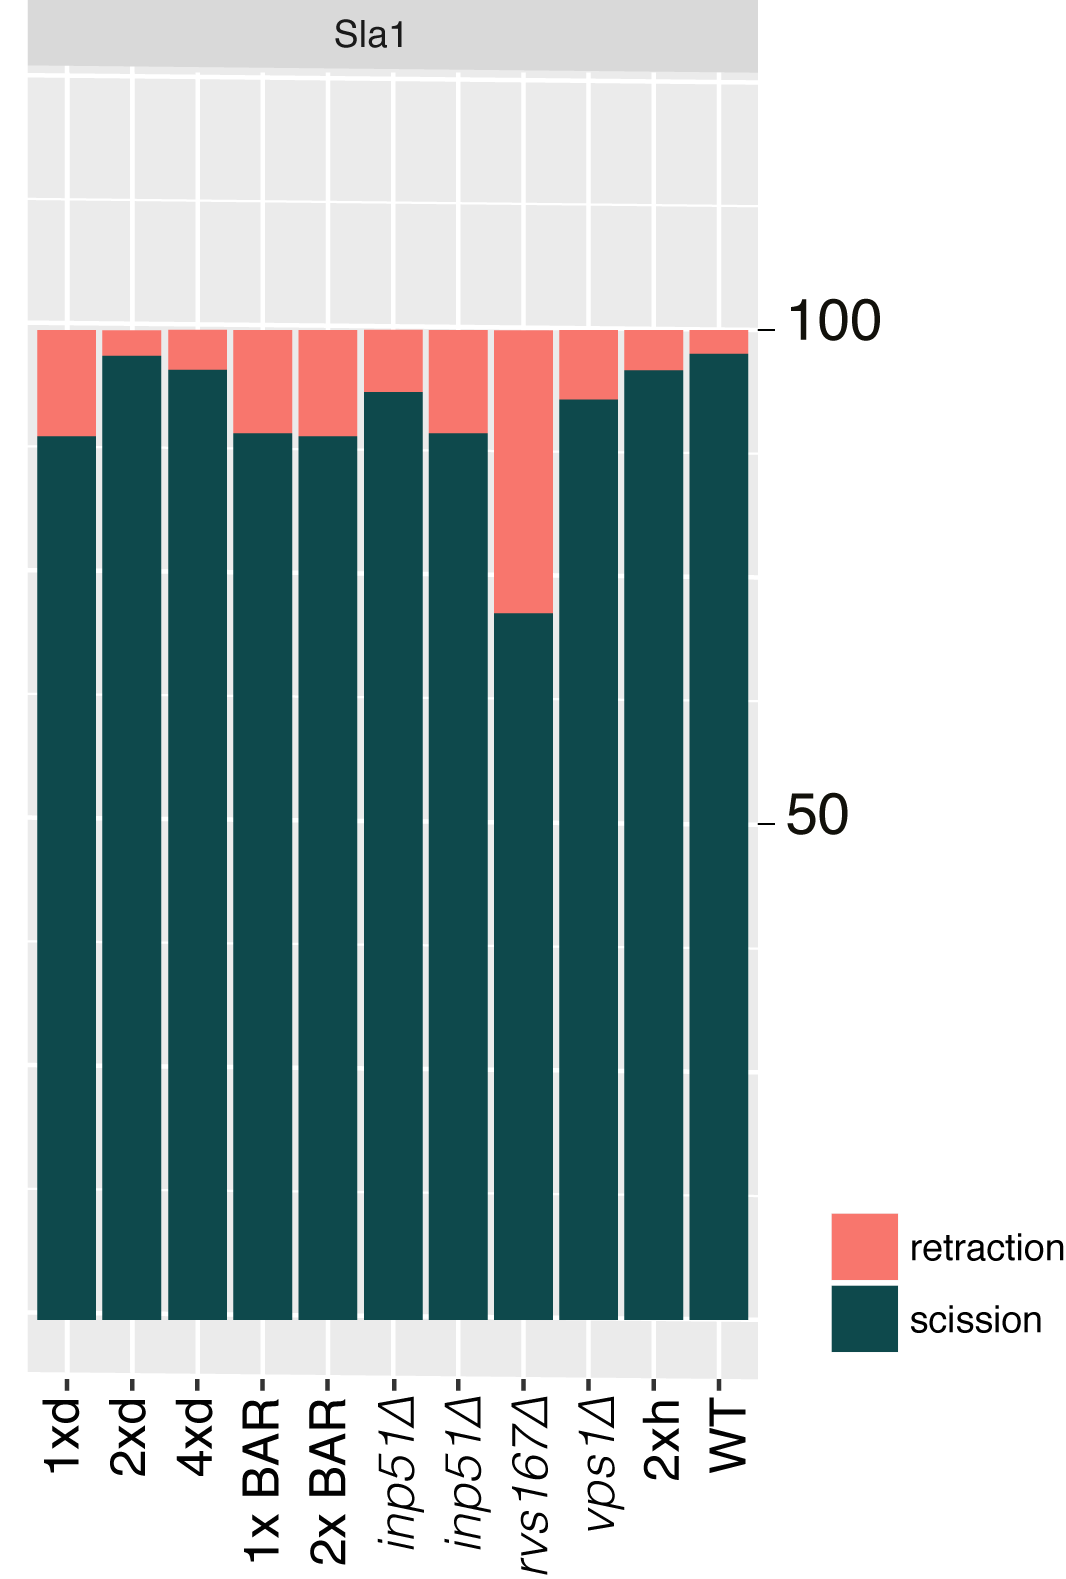
\includegraphics[scale=1]{figures/appendix/retraction_rates_all}
%\captionsetup{justification=raggedright,singlelinecheck=false,labelformat=empty}
%\captionsetup{justification=raggedright,singlelinecheck=false}
\caption[Scission failure rates]{Sla1-GFP retraction rates for various strains}
\end{figure}


\begin{figure}[H]
	\vspace{4cm}
%	\hspace{0.1cm}
	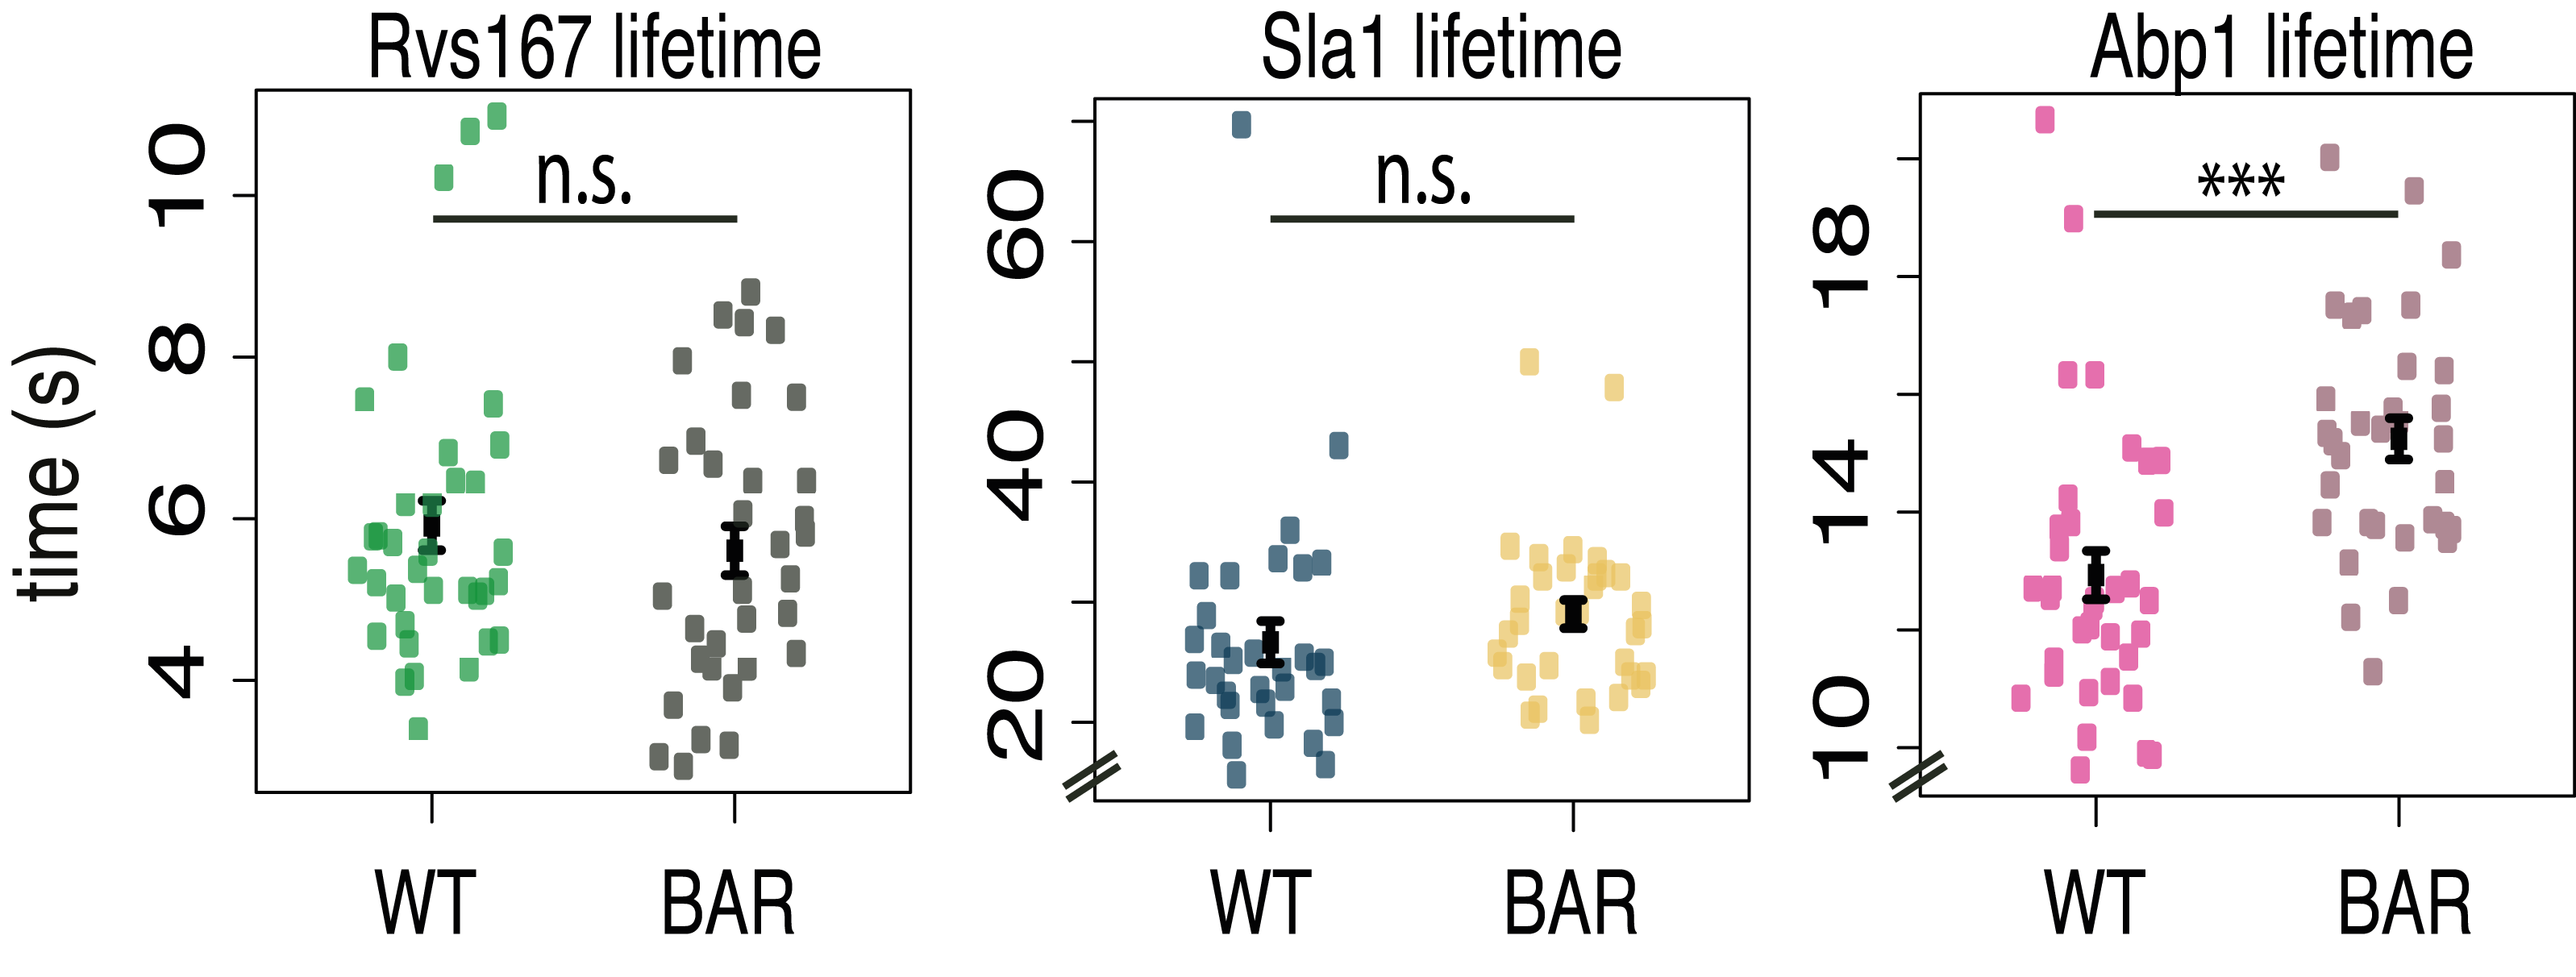
\includegraphics[scale=0.57]{figures/appendix/delsh3_5}
%	\captionsetup{labelformat=empty}
	\caption[Lifetimes of proteins in WT and BAR cells]
{ Lifetimes of proteins in WT and BAR cells measured by TIRF microscopy}
\end{figure}